\documentclass[12pt]{article}
\usepackage[utf8]{inputenc}
\usepackage{graphicx}
\usepackage{subcaption}
\usepackage{amsmath} 
\usepackage{fancyhdr} 
\usepackage{geometry} 
\usepackage{dirtytalk} 
\usepackage[english]{babel}
\usepackage{csquotes}
\usepackage{hyperref}
\usepackage{listings}
\lstset{
    language=C,
    basicstyle=\ttfamily, 
    numberstyle=\tiny,
    frame=single,
    breaklines=true,
}

\begin{document}
\begin{titlepage}
\begin{center}
    
\includegraphics[width=0.3\textwidth]{image.png} \\[0.2cm]
    
    \textbf{MINISTRY OF EDUCATION, CULTURE AND RESEARCH 
OF THE REPUBLIC OF MOLDOVA} \\[0.3cm]
    
    \textbf{Technical University of Moldova 
Faculty of Computers, Informatics and Microelectronics 
Department of Software and Automation Engineering} \\[2cm]
    
    \textbf{Postoronca Dumitru FAF-233}\\[0.5cm]
    
    \Huge \textbf{Report} \\[0.5cm]
    
    \large Individual Work №1\\[0.5cm]
    
    \textbf{of LFA} \\[3cm]
    
    \begin{flushright}
        \textit{Checked by:} \\
        \textbf{Cojuhari Irina}, \textit{university assistant} \\
        DISA, FCIM, UTM
    \end{flushright}
    
    \vfill
    
    Chișinău -- 2024
\end{center}
\end{titlepage}


\newpage
\setcounter{page}{1}
\pagestyle{fancy}
\fancyhf{}
\rhead{\thepage}
\lhead{FAF-233 Postoronca Dumitru ; Individual work №1}

\section*{Conditions of the Task}
\begin{enumerate}
    \item Create the alorithm for convertion of the given number from the keyboard to base 2, 8 and 16
Design a DFA or NFA (with or without e-transitions) that accepts all strings over the 
alphabet {\$,c,0,1,2,3,4,5,6,7,8,9,.} that correspond to valid currency amounts. A valid 
string is either a dollar sign followed by a number which has no leading 0's, and may have a 
decimal point in which case it must be followed by exactly two decimal digits, OR a one or two-digit amount 
followed by the cent sign c. The single exception to this rule is that strings which begin with "\$0." 
and are followed by exactly two digits are also acceptable. Thus, \$432.63, \$1, \$0.29, 47c, 2c are all 
accepted, but \$021, \$4.3, \$8.63c, \$0.0 are not accepted. 
    \item Find a grammar for a simple arithmetic expression in a 
      programming language, and show the 
      parse tree for sample expressions:

      Variant 25: \textbf{((a-b)+c)}
\end{enumerate}

\section*{Visual Solution}
\hspace{0.8cm}

I designed an NFA to represent the currency convertion
states. I tried to pass the test cases specified in condition through the NFA
and all of them passed.

\begin{figure}[!h]
\begin{center}
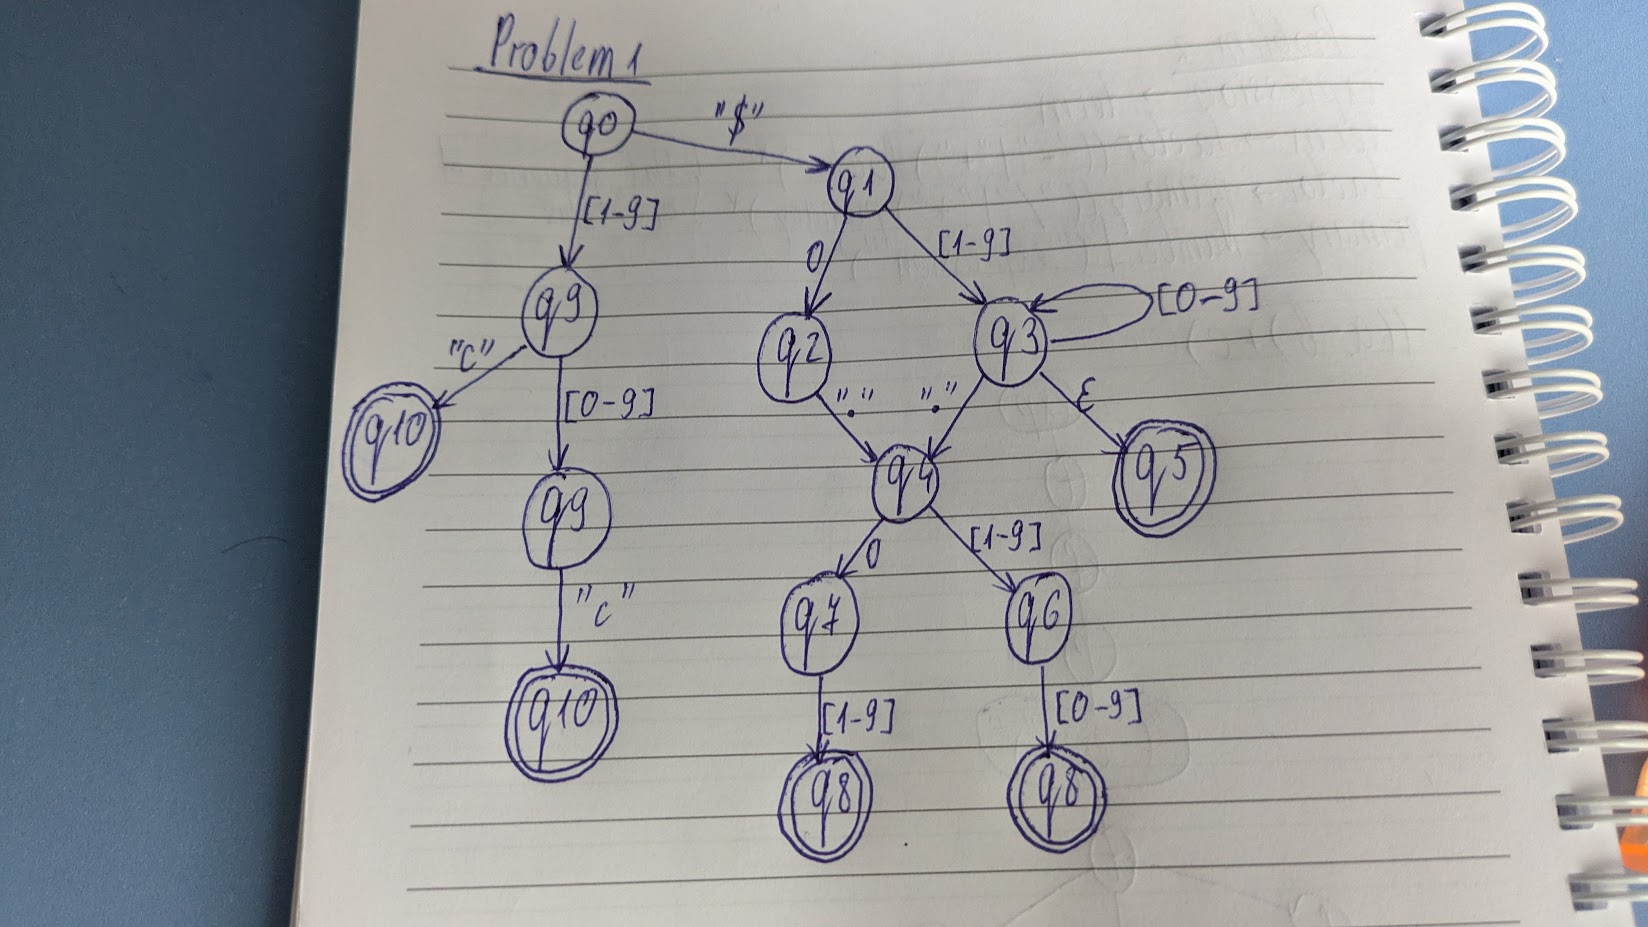
\includegraphics[width=0.72\textwidth]
{problem1.jpg}
\end{center}
\caption{NFA for currency convertion}
\label{fig:pic1}
\end{figure}

\clearpage
I specified the rules of the grammar and the parse tree below in Figure 2. You can see some uncommon
representations like ()*. This is uses to show that a node can contain as children multiple
factors/terms including only one factor/term with operations. As inspiration I use a good book where the author 
explain how to craft interpreters and take in consideration the edge 
cases \cite{interpreterref}

\begin{figure}[!h]
\begin{center}
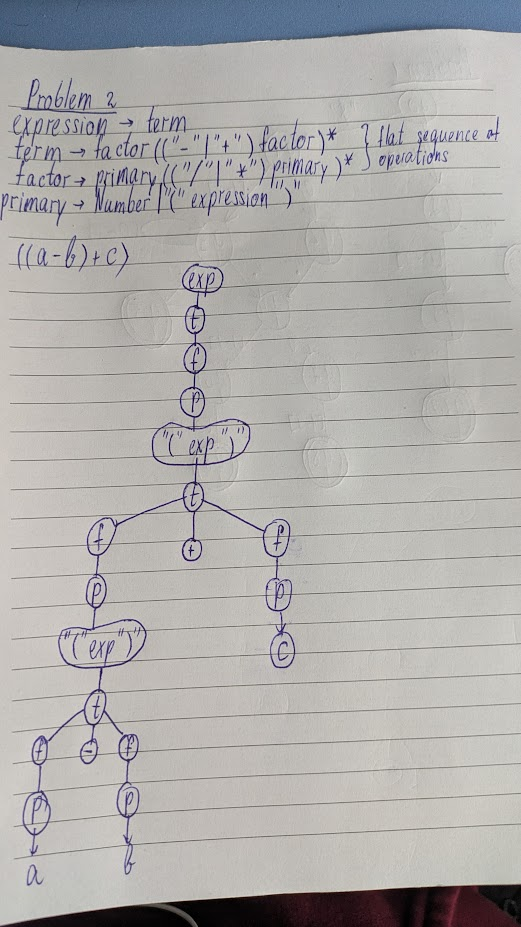
\includegraphics[width=0.5\textwidth]
{problem2.jpg}
\end{center}
\caption{Grammar and parse tree for the expression}
\label{fig:pic2}
\end{figure}

%\clearpage % Ensures that everything before this is placed first
Also in order to avoid ambiguity in priority of operations I specified \textit{term} rule and 
\textit{factor} rule


\section*{Conclusions}
\hspace{0.6cm} 
I learned during this individual work how to properly analyse how to 
build a NFA and to create a good grammar to suit algorithmic expressions. 
I tried to build a grammar suitable for all variants listed on ELSE and 
to build the parse tree for my variant.

\begin{thebibliography}{9}

  \bibitem{interpreterref}
  Robert Nystrom (2021) \emph{Crafting-Interpreters 
  \href{https://craftinginterpreters.com/parsing-expressions.html}{https://craftinginterpreters.com/}}
\end{thebibliography}
\end{document}
